\chapter{Effects of alloying elements on the elastic properties of bcc Ti-X alloys}

\section{Introduction}

The present chapter is aimed at studying the effects of alloying elements on the mechanical properties of Ti-alloys as well as completing a database to calculate the elastic properties as a funciton of composition. This is accomplished by systematically studying the single crystal elastic stiffness constants (c$_{ij}$'s) and polycrystalline aggregate properties of bcc Ti-X (X = Mo, Nb, Ta, Sn, Zr) alloys. The elastic properties are calculated using first-principles calculations based on density functional theory (DFT). The composition dependence of elastic properties of Ti-X alloys is explored through the dilute solutions and special quasirandom structures (SQS) \cite{Jiang2004} for concentrated solutions using the methodologies outlined in the methodoly chapter. The obtained elastic properties are then fit using the CALPHAD method and extrapolated to higher order Ti-alloys. 

\section{Modeling and Calculations}

\subsection{Calculation details}
In the present work the Vienna ab-initio Simulation Package (VASP) \cite{Kresse1996} was employed to calculate the elastic properties of pure elements and Ti-containing binary systems in the bcc phase. The ion-electron interactions were described using the projector augmented wave (PAW) \cite{Kresse1999,Blochl1994} method and based on the previous work of comparing X-C functionals (Figure \ref{Ch2-figure:PBEvsPW91}) the exchange-correlation functional of the generalized gradient approach depicted by Perdew, Burke, and Ernzerhof (PBE-GGA) was employed \cite{Perdew1996a}. Three magnitudes of strain were compared by doing the same calculations on the Ti-Mo system using the  $\pm$0.01, $\pm$0.013 and $\pm$0.007 magnitudes of strain. The three magnitudes of strain showed little variance in results, thus the calculations were done with PBE and $\pm$0.01 strains. For consistency, a 310 eV energy cutoff was adopted for all calculations, which is roughly 1.3 times higher than the default value. The energy convergence criterion was 10$^{-6}$ eV/atom, and the Monkhorst-Pack scheme is used for Brillouin zone sampling \cite{Kresse1996,Monkhorst1976a}. 

For the Ti-X binary systems, calculations for both dilute and SQS solutions were carried out. Three SQS cells with mole fractions of X atoms at 0.25, 0.5, and 0.75 were employed. Five dilute solutions were calculated for each Ti-X binary alloy using supercell sizes, i.e., Ti$_{53}$X (54-atom), Ti$_{15}$X (16-atom), Ti$_{7}$X (8-atom), X$_{15}$Ti (16-atom), and X$_{53}$Ti (54-atom). The interaction paramters for the  elastic stiffness constants were then determined according to the methodology laid out in chapter 2. 

\subsection{Modeling details}

  The first-principles results are then used to model the elastic stiffness constants. The modeling was completed by calculating the difference between the first-principles calculations and a linear extrapolation between pure elements. The differences were then used to fit to the interaction parameters. Due to the limitations within the PARROT module, a mathmatica script was used to fit the interaction parameters. The mathematica script is appended in appendix C. With the focus being Ti-rich alloys, the first-principles results with 70 at. \% Ti or higher were weighted heavier (x6, according to the authors' practices) than the other points for the fittings. The best fit was found by comparing the fittings obtained with one interaction parameter or with two interaction parameters. The moduli values were than calculated from the elastic stiffness constants according to Eq. Y in the methodology chapter.

\section{Results and discussion}

\subsection{Evaluation of calculation settings}

The X-C functionals of PW91 and PBE were tested on the Ti-Ta binary system. The results are plotted in Figure \ref{Ch5-figure:PBEvsPW91}. It is shown that the c$_{44}$ values of Ti-Ta alloys consistently differ around 10 GPa or less between the PW91 and PBE calculations. The c$_{11}$ and c$_{12}$ calculations differ less than 5 GPa. The c$_{11}$ and c$_{12}$ values with 25 at.$\%$ Ta from SQS calculations vary by 26 GPa and 13 GPa, respectively. Since overall the values vary by an error of less than 0.2 (calculated with Eq. Y), it is concluded that the X-C functional choice does not make a significant difference in the results. The PBE functional was created after PW91 and meant to be an improvement on the PW91 and was chosen for the present work. 

Three magnitudes of strain were tested on the Ti-Mo binary system and plotted in \ref{Ch5-figure:Strain}. The results show that the different strain magnitudes do not affect the results. For example, the data calculated using $\pm$0.01, $\pm$0.013, and $\pm$0.007 strains at Mo$_{15}$Ti for c$_{11}$ was 451 GPa, 450 GPa, and 450 GPa, respectively, varying within 1 GPa (< 1$\%$), similar to the variance in the c$_{12}$ and c$_{44}$ results. Overall, the variance in the c$_{11}$ and c$_{12}$ is less than 0.02 (Eq. Y). The largest variance is seen in the Ti$_{50}$Mo$_{50}$, the c$_{44}$ values are 42 GPa, 42 GPa, and 65 GPa calculated with $\pm$0.01, $\pm$0.013, and $\pm$0.007 strains, respectively. Overall, the strain magnitude does not seem to affect the calculated results, and the $\pm$0.01 strain magnitude is thus used for all the calculations.

\subsection{Calculations of the Ti-X elastic properties}

The elastic stiffness constants and bulk modulus \textit{B} are calculated from c$_{ij}$ of pure elements in the bcc structure and reported in \ref{Ch5-table:pureeleelas}. The results in the present work were all obtained at 0 $^\circ$K without considering the effect of zero-point vibrational energy as discussed in the section of methodology. The results for Mo, Nb and Ta, which are stable in the bcc structure at low temperatures, are compared with experimental data at temperatures specified in the table \cite{Dickinson1967a,Bolef1961} The error (Eq. Y) between the present results and previous results for Mo, Nb and Ta are 2.61, 7.5, and 4.25 $\%$, respectively \cite{Simmons1971b,Dickinson1967a,Bolef1961}. This discrepancy is partially due to the experimental values being obtained at higher temperatures than the calculations at 0 $^\circ$K. 

Ti and Zr are stable in the hcp structure at low temperatures, and Sn is stable in the body centered tetragonal and diamond structures at low temperatures. Due to the instability of Ti, Sn and Zr in the bcc structure at low temperatures, their elastic stiffness coefficients are compared with previous first-principles calculations at 0 $^\circ$K \cite{Shang2010b} used the PW91 functional, and the errors are 2.4, 52.8 and 5.1 $\%$, respectively. The differences are related to the instability of the bcc structure, the different exchange correlation functionals and the different input parameters chosen. Due to the bcc instability, multiple relaxation schemes were run in the present work to find the lowest energy structure retaining the bcc symmetry, making the results the most accurate representation of the bcc pure elements. 
 
Figure \ref{Ch5-figure:tixyoungs} summarizes the present Young's modulus results for each Ti-X binary system (circles). The solid lines are from the Voigt-Reuss-Hill approach with the elastic coefficients from the current modeling using Eq. Y and the model parameters shown in Table \ref{Ch5-table:tixelasip}. The Hill average is plotted as a solid black line while the Voigt (high bound) and Reuss (low bound) are plotted as dotted lines and dashed lines, respectively. When the structures are stable the Voigt and Reuss do not vary drastically but when the structures is unstable the Voigt and Reuss show the high and low bounds of the modulus calculations with the Hill average being what the database will predict. The results calculated for the Ti-Mo, Ti-Nb, and Ti-Ta systems are compared with previous calculated results from Ikehata et al. \cite{Ikehata2004}, and the difference is due to the different input parameters and structures used at each composition. Ikehata et al. used the s electrons as the valance electrons for Ti and used the B2 structure for their Ti$_{0.5}$X$_{0.5}$ with Ti at the body centered site and X at the corner site. For the Ti$_{0.25}$X$_{0.75}$ and Ti$_{0.75}$X$_{0.25}$ structures they used the DO$_3$ structure with space group $Fm\overline{3}m$, as opposed to the BCC space group of $Im\overline{3}m$. While the present work used the p electrons as valance for Ti based on updated work and new recommendations by VASP and 16-atom SQS structures from Jiang et al. \cite{Jiang2004}. The SQS structures mimic the random substitution of elements that represent the atomic structures of solution phases better. The Ti-Mo, Ti-Nb and Ti-Ta alloy results are also compared with available experimental results \cite{Zhang2015,Boyer1994,Sung2015,Ozaki2004,Fedotov1985,Zhou2009a,Zhou2004a} in Table \ref{Ch5-table:tixelasdata}. 

Figure \ref{Ch5-figure:tixyoungs}a compares the present results for the Ti-Mo alloy system with experimental data from Zhang et al. \cite{Zhang2015}, Collings et al. \cite{Boyer1994}, and Sung et al. \cite{Sung2015}. It can be seen that the Young's modulus increases from pure Ti to pure Mo. The results from Sung et al. \cite{Sung2015} differ by about 60 GPa from the present work. However, during the XRD and TEM investigations by Sung et al, one of the metastable phases, $\alpha$" and $\omega$, in addition to the bcc phase was observed in the samples. The $\omega$ phase is a hexagonal phase (space group P6/mmm) with lattice parameters closely matching those of the bcc phase, and the $\alpha$" phase is a martensitic orthorhombic phase (space group Cmcm). The formation of the $\alpha$" and $\omega$ phases causes variations in the mechanical properties and thus the mechanical properties are expected to vary from the elastic properties of the single bcc phase. Zhang et al. \cite{Zhang2015} and Collings et al. \cite{Boyer1994} did not observe the formation of either metastable phase. The Young's modulus determined by Zhang et al. and Collings et al. are predicted with the present Voigt-Reuss bounds but have an error of 0.39 (Eq. Y) from the Hill average Young's modulus. 

The present Young's moduli of the Ti-Nb alloy system are compared with data from Ozaki et al. \cite{Ozaki2004} and Collings et al. \cite{Boyer1994} in Figure \ref{Ch5-figure:tixyoungs}b, showing an increase in Young's modulus with an increase in Nb concentration. The analyses of the samples from the work by Ozaki et al. and Collings et al. showed that the alloys all contained the single bcc phase. The Young's modulus from the present first-principles calculations show an error of 0.09 (Eq. Y) from the Young's modulus determined by Ozaki et al. and Collings et al. 

The Young's modulus calculation results for the Ti-Ta alloy system are plotted in Figure \ref{Ch5-figure:tixyoungs}d. Figure \ref{Ch5-figure:tixyoungs}d also plots the Young's modulus values that were experimentally determined from Fedotov et al. \cite{Fedotov1985} and Zhou et al. \cite{Zhou2009a,Zhou2004a}. The present Young's moduli calculated have an error of 0.19 (Eq. Y) from the experimental Young's moduli determined by Fedotov et al and Zhou et al. The Young's modulus in the Ti-Ta alloy system increases from pure Ti to pure Ta. 

The error between the Young's moduli determined experimentally and the Young's moduli calculated using DFT is expected due to the temperature difference (calculations at 0 $^\circ$K and experiments at 298 $^\circ$K). The Young's modulus results determined experimentally fit well within the Voigt and Reuss bounds and the present calculations provide good prediction of the elastic properties of the Ti-Mo, Ti-Nb and Ti-Ta alloys as a function of composition.

For the Young's modulus of the Ti-Sn (Figure \ref{Ch5-figure:tixyoungs}c) and Ti-Zr (Figure \ref{Ch5-figure:tixyoungs}e)  systems there is no experimental data to compare with due to the instability in the bcc phase. For the Ti-Sn alloy system the Young's modulus increases until around 35 at \% Sn when the Young's modulus than decreases to pure Sn. The Young's modulus data, for the Ti-Zr alloy system, increases up to 40 at.\% Zr, and then the Young's modulus decreases to pure Zr. Figure \ref{Ch5-figure:tixmap} plots the Young's modulus as a function of composition from pure Ti in the bcc structure to the alloying element (X = Mo, Nb, Sn, Ta, Zr) to be able to compare the effects of each alloying element on the Young's modulus.

Figure \ref{Ch5-figure:tixc11} to Figure \ref{Ch5-figure:tixc44} plots the calculated elastic stiffness constants, $\overline{C}_{11}$, $\overline{C}_{12}$, $\overline{C}_{44}$ (circles) and compares it with the elastic stiffness constants fitting (solid line) and linear extrapolation between the pure elements for each binary alloy, Ti-Mo, Ti-Nb, Ti-Sn, Ti-Ta, and Ti-Zr. The previous results from Ikehata et al. \cite{Ikehata2004} are plotted for comparison for the Ti-Mo, Ti-Nb, and Ti-Ta alloys. The trend seen in the elastic stiffness constants data depict that Mo, Nb and Ta affect the elastic stiffness constants in a similar fashion. As shown in Figure \ref{Ch5-figure:tixc11}a, b and d the  i$\overline{C}_{11}$ increases from Ti to X (Mo, Nb, Ta) and in Figure \ref{Ch5-figure:tixc44}a, b and d the  $\overline{C}_{44}$ values first decrease and then increase with the addition of the alloying element Mo, Nb and Ta respectively. The calculated $\overline{C}_{12}$ increases by the addition of Mo and Ta (Figure \ref{Ch5-figure:tixc12}a and Figure \ref{Ch5-figure:tixc12}d, respectively), and the $\overline{C}_{44}$  first decreases and then increases by the addition of Nb (Figure \ref{Ch5-figure:tixc12}b). A similar trend is shown in the $\overline{C}_{11}$ and $\overline{C}_{12}$ data for the Ti-Sn system (Figure \ref{Ch5-figure:tixc11}c and Figure \ref{Ch5-figure:tixc12}c). The $\overline{C}_{11}$ and $\overline{C}_{11}$ values increase and then decrease from pure Ti to pure Sn. The trend of the  $\overline{C}_{44}$ seen in Figure \ref{Ch5-figure:tixc44}c increases, decreases, and then increases from pure Ti to pure Sn. In the Ti-Zr system, the $\overline{C}_{11}$ and $\overline{C}_{44}$ values increase and then decrease with increasing Zr concentration (Figure \ref{Ch5-figure:tixc11}e and Figure \ref{Ch5-figure:tixc44}e). The calculated $\overline{C}_{12}$ values for the Ti-Zr system decrease and then increase shown in Figure \ref{Ch5-figure:tixc12}e.

The instability in the bcc phase can be seen from Figure \ref{Ch5-figure:tixc11-c12}, which shows the $\overline{C}_{11}$ - $\overline{C}_{12}$ values from first-principles calculations and the present modeling. The bcc phase is mechanical unstable at concentrations less than 5.5, 11.5, 51.5, 9.5 and 4.0 at. \% for Mo, Nb, Sn, Ta and Zr, respectively. Figure \ref{Ch5-figure:tixbulk} and Figure \ref{Ch5-figure:tixshear} show the bulk and shear moduli plotted similarly to the Young's modulus in Figure \ref{Ch5-figure:tixyoungs} with the present results (circles), the Hill average (solid black line), and Voigt (purple dashed line) and Reuss (yellow dashed line) bounds. Similar trends in the \textit{B} and \textit{G} data are seen for the Ti-Mo, Ti-Nb and Ti-Ta systems. The \textit{B} and \textit{G} increase with increasing Mo, Nb and Ta concentration, as shown in Figure \ref{Ch5-figure:tixbulk} and Figure \ref{Ch5-figure:tixshear}, respectively.  The bulk and shear moduli values increase and then decrease from pure Ti to pure Sn in the Ti-Sn system (Figure \ref{Ch5-figure:tixbulk}c and Figure \ref{Ch5-figure:tixshear}c). In the Ti-Zr system, the \textit{B} decreases from pure Ti to pure Zr (Figure \ref{Ch5-figure:tixbulk}e) and the \textit{G} first increases and then decreases from pure Ti to pure Zr (Figure \ref{Ch5-figure:tixshear}e). 

\subsection{Extrapolation to ternary and higher ordered systems}

The interaction parameters in Table \ref{Ch5-table:tixelasip} can be used to predict the elastic stiffness constants of higher order Ti-alloys by summing the interaction parameters of each binary alloy contained in the multi-component alloy from Eq. Y. The predicted elastic stiffness constants of the multi-component alloys can be used to calculate Young's modulus as a function of composition as shown in Figure \ref{Ch5-figure:tixmap}. The Hill average is plotted as solid lines while the Voigt and Reuss bounds are plotted as dotted and dashed lines, respectively. The accuracy of prediction of the elastic properties of higher ordered Ti alloys can be evaluated by comparing the predicted results with previous experimental results \cite{Niinomi2012,Tane2010a,Geetha2009,Mohammed2014} as shown in Figure \ref{Ch5-figure:tixdatabase} and Table \ref{Ch5-table:tixdatacomp}. The black diagonal line represents a perfect correlation between the predicted and experimental Young's modulus. The grey region is the error (3 GPa) in the first-principles calculations. The error in the first-principles is the average variance in $\overline{C}_{11}$, $\overline{C}_{12}$, and $\overline{C}_{44}$ from Eq. Y-Eq. Y. 

As it can be seen, the difference between experimental Young's modulus at the same composition from Niinomi et al. \cite{Niinomi2012}, Geetha et al. \cite{Geetha2009}, Tane et al. \cite{Tane2010a} and Mohammad et al. \cite{Mohammed2014} varies from 2 GPa to 46 GPa based on the heat treatments and measuring techniques. The scattering in the Young's modulus among experimental measurements is denoted by the vertical error bars in Figure \ref{Ch5-figure:tixdatabase}. The horizontal error bars show the Reuss and Voigt Young's modulus ranges with the Hill average marked by the circle. The experimental Young's moduli vary from the present predictions anywhere from 0.69 to 14 GPa. This difference is partially due to the temperature difference between the first-principles data and the experimental results. Considering the fact that the experimental results at the same composition vary drastically, the first-principles calculations give a good representation of the elastic properties of higher order Ti-alloys. Introducing the binary interaction parameters of non-Ti containing alloys in the system and the ternary interaction parameters can further improve the database predictions.

\section{Conclusion}

The effects of five alloying elements on the elastic properties of bcc Ti-X (X = Mo, Nb, Sn, Ta, Zr) alloys, including the elastic stiffness constants, bulk modulus, shear modulus, and Young's modulus, were systematically studied using first-principles calculations. The CALPAHD methodology was used to evaluate interaction parameters so that the elastic properties can be predicted as a function of composition. The present calculations showed that 5.5 at.$\%$, 11.5 at.$\%$, 51.5 at.$\%$, 9.5 at.$\%$ and 4.0 at.$\%$ of Mo, Nb, Sn, Ta and Zr, respectively, were needed to stabilize the bcc phase according to the Born criteria. The trends observed were summarized for each Ti-X (X= Mo, Nb, Sn, Ta, Zr) binary system. Alloying with Mo, Nb and Ta showed to produce similar trends which is presumably due to Mo, Nb, and Ta being stable in the bcc structure at room temperature and being strong bcc stabilizers. The interaction parameters determined in the current work were used to predict the elastic properties of higher order alloys. The accuracy of database predictions of the Young's modulus was determined by comparing with the calculated and experimental Young's moduli. Overall, the database provides good predictions of the elastic properties of Ti-alloys in the bcc phase as a function of composition. To improve the database predictions, the non-Ti containing binary interaction parameters and the ternary interactions parameters should be determined.

\newpage
\begin{table}[H]
	\caption{Calculated pure element elastic stiffness constants and the bulk modulus \textit{B} (in GPa) by X-C functional of PBE are compared with the previous first-principles calculations (FP) by X-C functional PW91 and experiments (Expt). Sv, pv and d refereeing to the s, p, and d states being treated as valance, respectively.}
	\centering
	\begin{tabular}{ c c c c c c }
		\hline
		Pure Elements & & $\bar{C}_{11}$ & $\bar{C}_{11}$  & $\bar{C}_{11}$ & \textit{B}\\
		\hline
		Ti$\_$sv & This work 0 K & 93 & 115 & 41 & 108\\
		& Calc 0 K \cite{Shang2010b} & 96 & 116 & 40 & 107\\
		Mo$\_$pv & This work 0 K & 475 & 164 & 108 & 268\\
		& Expt 73 K \cite{Simmons1971b} & 473 & 156 & 111 &\\
		& Expt 300 K \cite{Dickinson1967a} & 473 & 160 & 109 & 261\\
		Nb$\_$sv & This work 0 K & 245 & 144 & 27 & 178\\
		& Expt 4 K \cite{Simmons1971b} & 253 & 133 & 31 & \\
		& Expt 300 K \cite{Bolef1961} & 247 & 135 & 29 & 172\\
		Sn$\_$d & This work 0 K & 50 & 52 & 29 & 51\\
		& Calc 0 K \cite{Shang2010b} & 30 & 60 & 18 & 48\\
		Ta$\_$pv & This work 0 K & 278 & 164 & 81 & 202\\
		& Expt 0 K \cite{Simmons1971b} & 266 & 158 & 87 & \\
		& Expt 300 K \cite{Bolef1961} & 267 & 161 & 83 & 196\\
		Zr$\_$sv & This work 0 K & 86 & 91 & 32 & 89\\
		& Calc 0 K \cite{Shang2010b} & 82 & 94 & 30 & 90\\
		\hline
	\end{tabular}
	\label{Ch5-table:pureeleelas}
\end{table}
\clearpage
%%%

\newpage
\begin{table}[H]
	\caption{Evaluated interaction parameters $L_0$ and $L_1$ using the R-K polynomial Eq. Y for the elastic stiffness constants for the Ti-X binary systems.}
	\centering
	\begin{tabular}{ c c c c c c c }
		\hline
		Alloy & Interaction Parameter & Ti-Mo & Ti-Nb & Ti-Sn & Ti-Ta & Ti-Zr\\
		\hline
		$\bar{C}_{11}$ & $L_0$ & -22.16 & 40.46 & 119.46 & 83.65 & 246.97\\
		& $L_1$ & 0 & 0 & 0 & -67.76 & -135.95\\
		$\bar{C}_{12}$ & $L_0$ & -36.40 & -32.39 & 15.90 & 38.05 & -110.53\\
		& $L_1$ & 0 & 0 & -146.80 & 0 & 78.00\\
		$\bar{C}_{44}$ & $L_0$ & -142.9 & -41.54 & 59.79 & -51.96 & 70.06\\
		& $L_1$ & 0 & -41.95 & -94.38 & 0 & 0\\	
		\hline
	\end{tabular}
	\label{Ch5-table:tixelasip}
\end{table}
\clearpage
%%%

\newpage
\begin{longtable}[H]{ c c c c c c c c}
	\caption{First-principles calculations of the elastic stiffness constants, bulk modulus \textit{B}, shear modulus \textit{G}, and Young's modulus \textit{E} in GPa for different atomic percent compositions of the bcc Ti-X binary systems at 0 $^\circ$K. As well as experimental data for the Young's modulus obtained at 300 $^\circ$K by the reference stated.} 	\label{Ch5-table:tixelasdata} \\
	\hline
	Reference & Ti$_{1-b}$X$_b$ & $\overline{C}_{11}$ & $\overline{C}_{11}$ & $\overline{C}_{11}$ & \textit{B} & \textit{G} & \textit{E}\\
	\hline
	\endhead
	\hline
	\endfoot
	This work & Ti & 93 & 115 & 41 & 108 & -12.91 & -40.34\\
	This work & TiMo$_{6.3}$ & 124 & 111 & 38 & 115 & 20 & 54\\
	This work & TiMo$_{12.5}$ & 146 & 113 & 29 & 124 & 23 & 65\\
	This work & TiMo$_{25}$ & 178 $\pm$3 & 123 $\pm$15 & 32 $\pm$11 & 141 $\pm$15 & 30 $\pm$15 & 84 $\pm$15\\
	This work & TiMo$_{50}$ & 268 $\pm$9 & 136 $\pm$19 & 42 $\pm$9 & 180 $\pm$19 & 51 $\pm$19 & 138 $\pm$19\\
	This work & TiMo$_{75}$ & 385 $\pm$9 & 146 $\pm$6 & 66 $\pm$6 & 226 $\pm$9 & 84 $\pm$9 & 224 $\pm$9\\
	This work & TiMo$_{93.8}$ & 451 & 158 & 96 & 256 & 114 & 397\\
	This work & TiMo$_{98.1}$ & 464 & 163 & 100 & 263 & 118 & 308\\
	This work & Mo & 475 & 164 & 108 & 268 & 125 & 325\\
	Expt 300 K \cite{Zhang2015} & TiMo$_8$ & & & & & & 83\\
	Expt 300 K \cite{Zhang2015} & TiMo$_{12}$ & & & & & & 90\\
	Expt 300 K \cite{Boyer1994} & TiMo$_{8}$ & & & & & & 84\\
	Expt 300 K \cite{Boyer1994} & TiMo$_{11}$ & & & & & & 89\\
	Expt 300 K \cite{Boyer1994} & TiMo$_{18}$ & & & & & & 101\\
	This work & TiNb$_{1.9}$ & 93 & 115 & 35 & 108 & -18 & -56\\
	This work & TiNb$_{12.5}$ & 116 & 116 & 37 & 116 & 11 & 31\\
	This work & TiNb$_{25}$ & 140 $\pm$11 & 116 $\pm$13 & 34 $\pm$10 & 124 $\pm$13 & 22 $\pm$13 & 63 $\pm$13\\
	This work & TiNb$_{50}$ & 181 $\pm$9 & 121 $\pm$2 & 31 $\pm$10 & 141 $\pm$9 & 31 $\pm$10 & 86 $\pm$10\\
	This work & TiNb$_{75}$ & 208 $\pm$3 & 130 $\pm$4 & 15 $\pm$10 & 156 $\pm$4 & 22 $\pm$10 & 64 $\pm$10\\
	This work & TiNb$_{93.8}$ & 242 & 134 & 18 & 170 & 28 & 81\\
	This work & TiNb$_{98.1}$ & 242 & 134 & 18 & 170 & 28 & 81\\
	This work & Nb & 245 & 144 & 27 & 178 & 35 & 98\\
	Expt 300 K \cite{Ozaki2004} & TiNb$_{29}$ & & & & & & 67\\
	Expt 300 K \cite{Ozaki2004} & TiNb$_{34}$ & & & & & & 74\\
	Expt 300 K \cite{Ozaki2004} & TiNb$_{44}$ & & & & & & 84\\
	Expt 300 K \cite{Boyer1994} & TiNb$_{26}$ & & & & & & 64\\
	Expt 300 K \cite{Boyer1994} & TiNb$_{30}$ & & & & & & 65\\
	Expt 300 K \cite{Boyer1994} & TiNb$_{34}$ & & & & & & 73\\
	Expt 300 K \cite{Boyer1994} & TiNb$_{44}$ & & & & & & 83\\
	This work & TiSn$_{6.3}$ & 100 & 122 & 46 & 115 & -10 & -30\\
	This work & TiSn$_{25}$ & 105 $\pm$5 & 114 $\pm$2 & 60 $\pm$4 & 111 $\pm$5 & 11 $\pm$5 & 31 $\pm$5\\
	This work & TiSn$_{50}$ & 88 $\pm$9 & 93 $\pm$9 & 46 $\pm$4 & 91 $\pm$9 & 10 $\pm$9 & 29 $\pm$9\\
	This work & TiSn$_{75}$ & 92 $\pm$9 & 55 $\pm$7 & 35 $\pm$8 & 67 $\pm$9 & 27 $\pm$9 & 72 $\pm$9\\
	This work & Sn & 50 & 52 & 29 & 51 & 7 & 21\\
	This work & TiTa$_{1.9}$ & 100 & 115 & 39 & 110 & -3 & -9\\
	This work & TiTa$_{6.3}$ & 116 & 113 & 30 & 114 & 11 & 32\\
	This work & TiTa$_{12.5}$ & 120 & 121 & 39 & 121 & 11 & 32\\
	This work & TiTa$_{25}$ & 167 $\pm$1 & 140 $\pm$3 & 45 & 149 $\pm$3 & 28 $\pm$3 & 78 $\pm$3\\
	This work & TiTa$_{50}$ & 208 $\pm$1 & 159 & 51 $\pm$3 & 175 $\pm$1 & 38 $\pm$3 & 106 $\pm$3\\
	This work & TiTa$_{75}$ & 239 $\pm$7 & 143 $\pm$5 & 62 $\pm$3 & 175 $\pm$7 & 56 $\pm$7 & 152 $\pm$7\\
	This work & TiTa$_{93.8}$ & 257 & 158 & 72 & 191 & 62 & 168\\
	This work & TiTa$_{98.1}$ & 264 & 163 & 72 & 197 & 62 & 169\\
	This work & Ta & 278 & 164 & 81 & 202 & 70 & 189\\
	Expt 300 K \cite{Fedotov1985} & TiTa$_{38}$ & & & & & & 62\\
	Expt 300 K \cite{Fedotov1985} & TiTa$_{42}$ & & & & & & 79\\
	Expt 300 K \cite{Fedotov1985} & TiTa$_{48}$ & & & & & & 95\\
	Expt 300 K \cite{Zhou2004a} & TiTa$_{38}$ & & & & & & 67\\
	Expt 300 K \cite{Zhou2004a} & TiTa$_{51}$ & & & & & & 105\\
	This work & TiZr$_{1.9}$ & 112 & 106 & 43 & 108 & 17 & 48\\
	This work & TiZr$_{25}$ & 148 $\pm$14 & 82 $\pm$7 & 54 $\pm$7 & 104 $\pm$14 & 44 $\pm$14 & 116 $\pm$14\\
	This work & TiZr$_{50}$ & 152 $\pm$17 & 76 $\pm$12 & 48 $\pm$12 & 101 $\pm$17 & 44 $\pm$17 & 115 $\pm$17\\
	This work & TiZr$_{75}$ & 126 $\pm$12 & 82 $\pm$3 & 45 $\pm$3 & 97 $\pm$12 & 34 $\pm$12 & 91 $\pm$12\\
	This work & TiZr$_{93.8}$ & 89 & 90 & 34 & 90 & 9 & 27\\
	This work & Zr & 86 & 91 & 32 & 89 & 6 & 16\\
	\hline
\end{longtable}
%%%

\newpage
\begin{table}[H]
	\caption{Predicted Young's modulus (in GPa) of higher order alloys in the bcc phase compared to experimental values found with both the weight percent and atomic percent listed. The predicted Young's modulus was found using the pure elements and binary interaction parameter data.}
	\centering
	\begin{tabular}{ c c c c }
		\hline
		Alloy Name ($\%$wt) & at \% & Calc \textit{E} & Expt \textit{E}\\
		\hline
		Ti-35Nb-7Zr-5Ta \cite{Geetha2009} & Ti-24Nb-5Zr-2Ta & 81 & 80\\
		Ti-29Nb-13Ta-4.6Zr \cite{Geetha2009}  & Ti-20Nb-5Ta-3Zr & 76 & 75\\
		Ti-29Nb-13Ta-6Sn \cite{Geetha2009} & Ti-21Nb-5Ta-3Sn & 68 & 74\\
		Ti-29Nb-13Ta-4.6Sn \cite{Geetha2009} & Ti-20Nb-5Ta-3Sn & 67 & 66\\
		Ti-29Nb-13Ta-4.5Zr \cite{Geetha2009} & Ti-20Nb-5Ta-3Zr & 76 & 65\\
		Ti-29Nb-13Ta-4.6Zr \cite{Tane2010a} & Ti-21Nb-5Ta-3Zr & 76 & 64\\
		Ti-30Nb-10Ta-5Zr \cite{Tane2010a} & Ti-23Nb-4Ta-3Zr & 77 & 64\\
		Ti-35Nb-10Ta-5Zr \cite{Tane2010a} & Ti-25Nb-4Ta-4Zr & 80 & 65\\
		Ti-24Nb-4Zr-7.9Sn \cite{Mohammed2014} & Ti-15Nb-3Zr-4Sn & 65 & 54\\
		Ti–35Nb–2Ta–3Zr \cite{Mohammed2014} & Ti-23Nb-1Ta-2Zr & 69 & 61\\
		Ti-29Nb-11Ta-5Zr \cite{Mohammed2014} & Ti-20Nb-6Ta-2Zr & 74 & 60\\
		Ti-10Zr-5Ta-5Nb \cite{Mohammed2014} & Ti-6Zr-1Ta-3Nb & 64 & 52\\
		Ti-29Nb-13Ta-2Sn \cite{Mohammed2014} & Ti-20Nb-5Ta-1Sn & 66 & 62\\
		\hline
	\end{tabular}
	\label{Ch5-table:tixdatacomp}
\end{table}
\clearpage
%%%

\pagebreak
\begin{figure}[H]
	\centering
	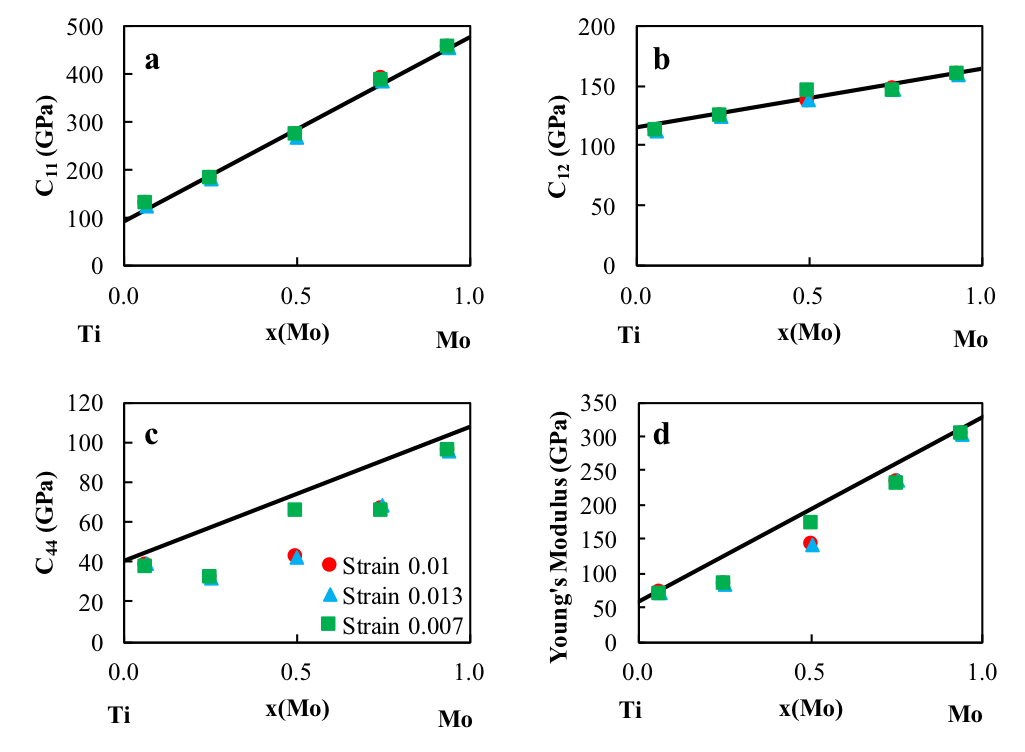
\includegraphics[width=\textwidth]{Chapter-5/Figures/Strain.png}
	\caption{Elastic stiffness constants for the bcc Ti-Mo binary system calculated with strains, 0.01, 0.03 and 0.07, respectively, showing comparable results.}
	\label{Ch5-figure:Strain}
\end{figure}

\pagebreak
\begin{figure}[H]
	\centering
	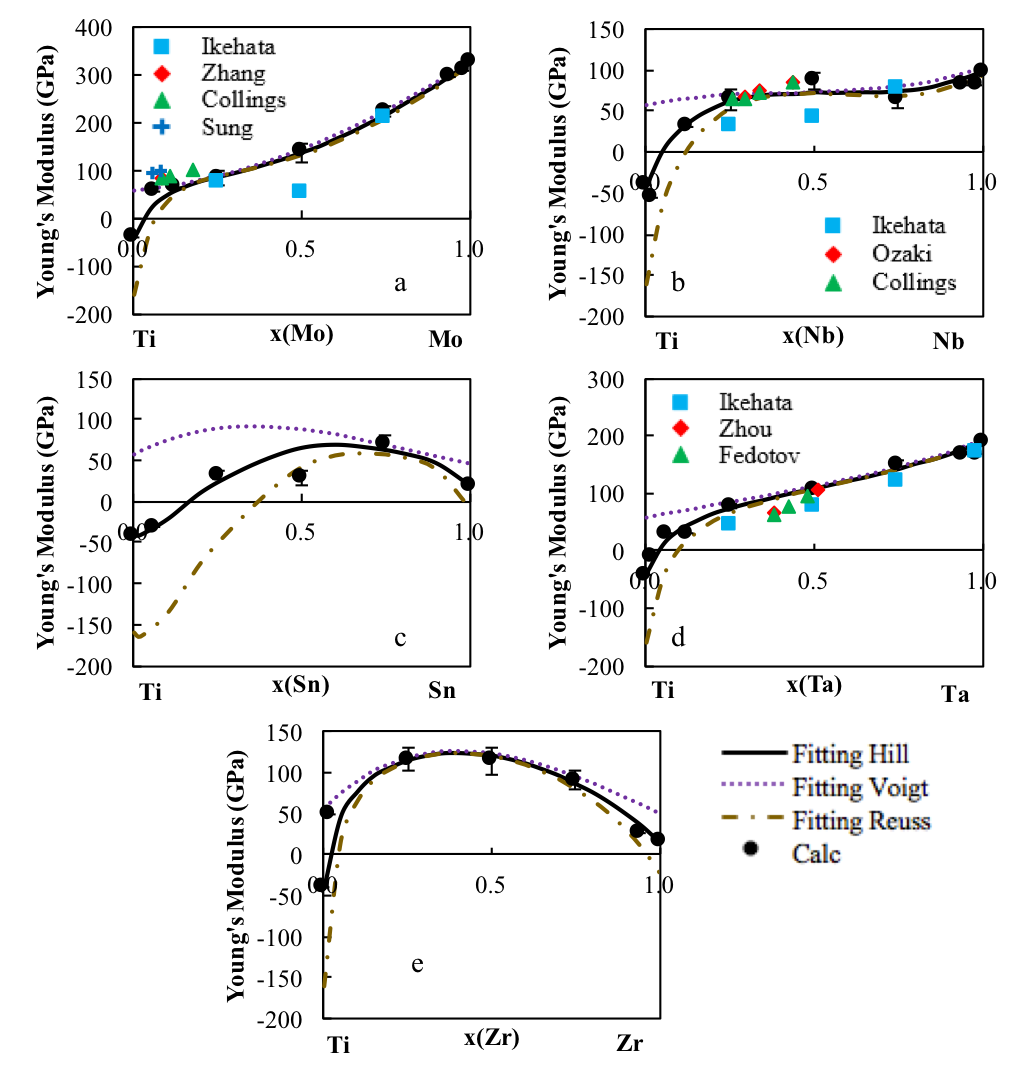
\includegraphics[width=\textwidth]{Chapter-5/Figures/tixyoungs.png}
	\caption{Young's modulus \textit{E} of the Ti-X binary systems. The present calculations are plotted as the filled circles with the error bars. The dotted purple line is the Voigt upper Young's modulus bound, the gold dot dashed line is the lower Reuss Young's modulus bound and the black line is the Hill Young's modulus average. The experimental values \cite{Ikehata2004,Zhang2015,Boyer1994,Sung2015,Ozaki2004,Fedotov1985,Zhou2009a,Zhou2004a,Friak2012,Wu2010a} are also included for comparison. }
	\label{Ch5-figure:tixyoungs}
\end{figure}

\pagebreak
\begin{figure}[H]
	\centering
	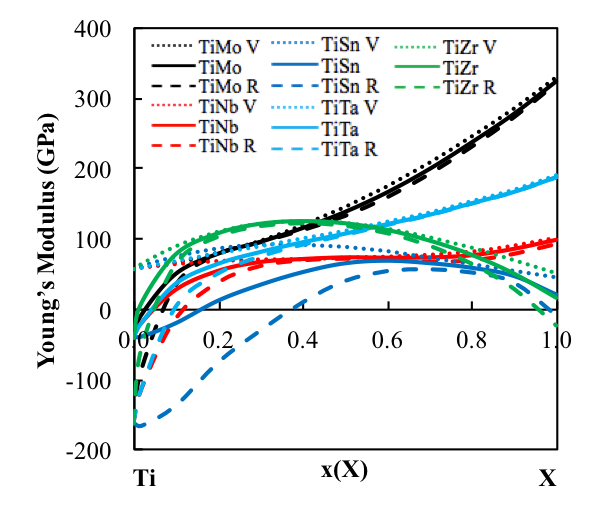
\includegraphics[width=\textwidth]{Chapter-5/Figures/emap.png}
	\caption{Young's modulus calculated from the model parameters (see \ref{Ch5-table:elasip}) and Eq. Y as a function of composition from bcc Ti to bcc X.}
	\label{Ch5-figure:tixmap}
\end{figure}

\pagebreak
\begin{figure}[H]
	\centering
	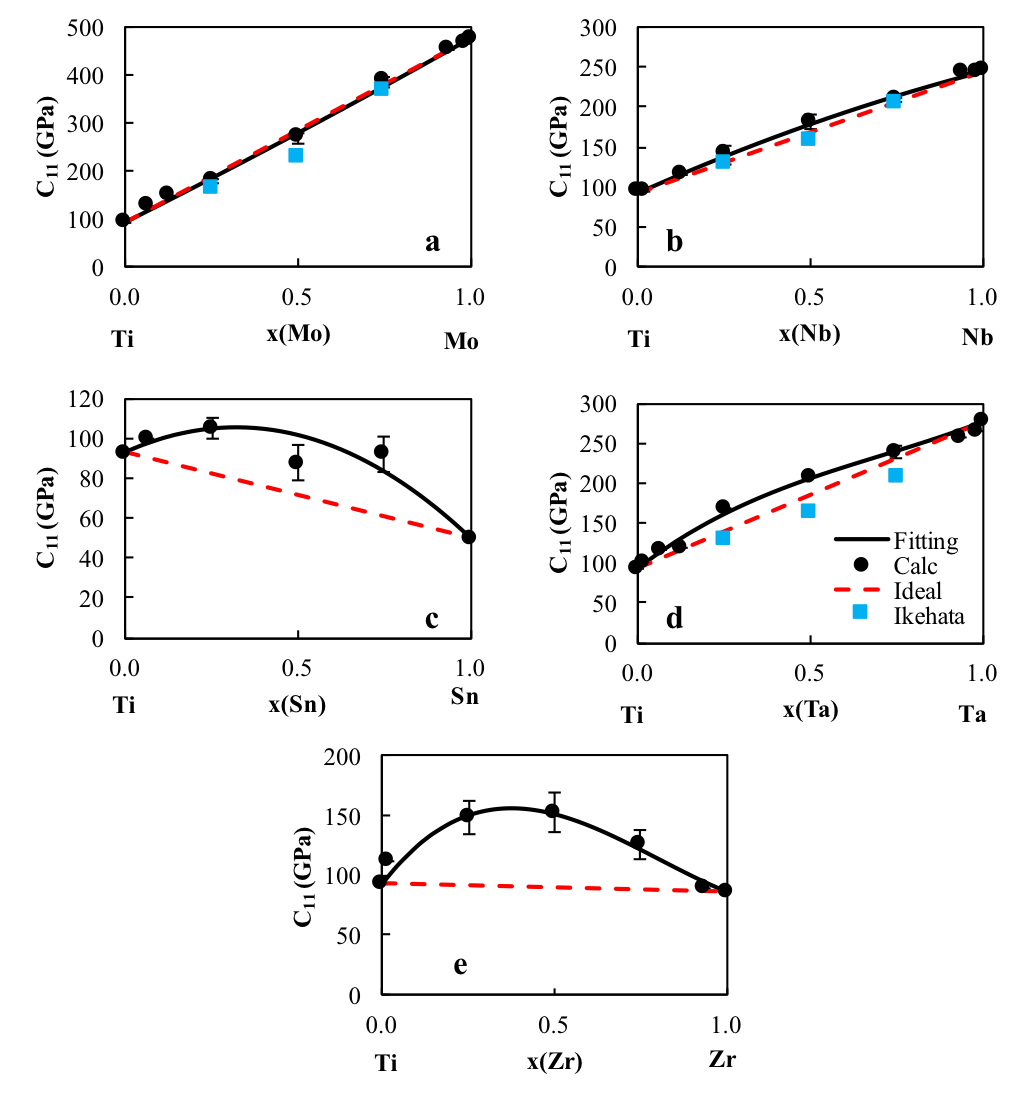
\includegraphics[width=\textwidth]{Chapter-5/Figures/tixc11.png}
	\caption{Calculated $\overline{C}_{11}$ values (circles) plotted with their errors as well as the pure element extrapolation (red dashed line) and the present modeling (black dashed line) for five Ti-X binary systems (X = Mo, Nb, Ta, Sn, Zr). Ti-Mo, Ti-Nb, and Ti-Ta alloys are compared with previous calculations from Ikehata et al. \cite{Ikehata2004}.}
	\label{Ch5-figure:tixc11}
\end{figure}

\pagebreak
\begin{figure}[H]
	\centering
	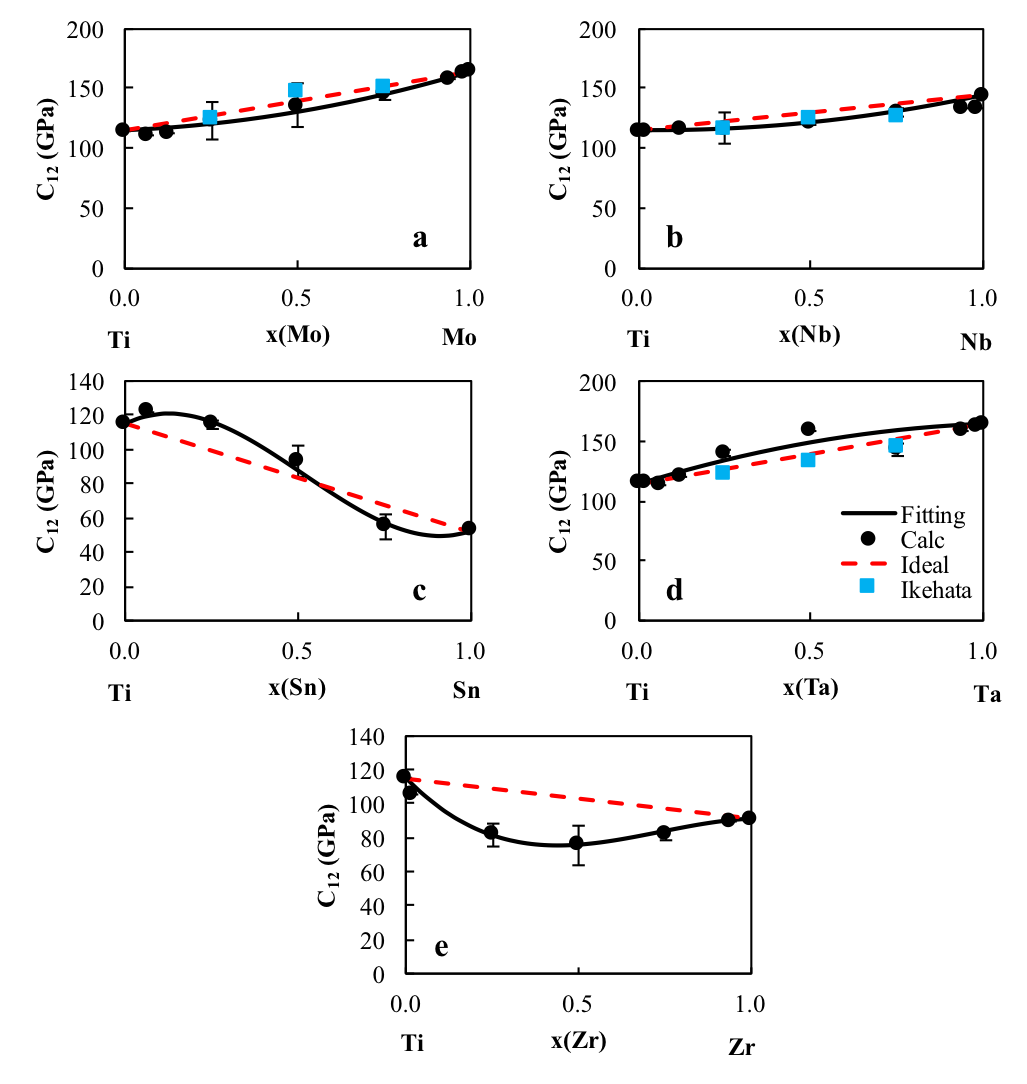
\includegraphics[width=\textwidth]{Chapter-5/Figures/tixc12.png}
	\caption{Calculated $\overline{C}_{12}$ values (circles) plotted with their errors as well as the pure element extrapolation (red dashed line) and the present modeling (black dashed line) for five Ti-X binary systems (X = Mo, Nb, Ta, Sn, Zr). Ti-Mo, Ti-Nb, and Ti-Ta alloys are compared with previous calculations from Ikehata et al. \cite{Ikehata2004}.}
	\label{Ch5-figure:tixc12}
\end{figure}

\pagebreak
\begin{figure}[H]
	\centering
	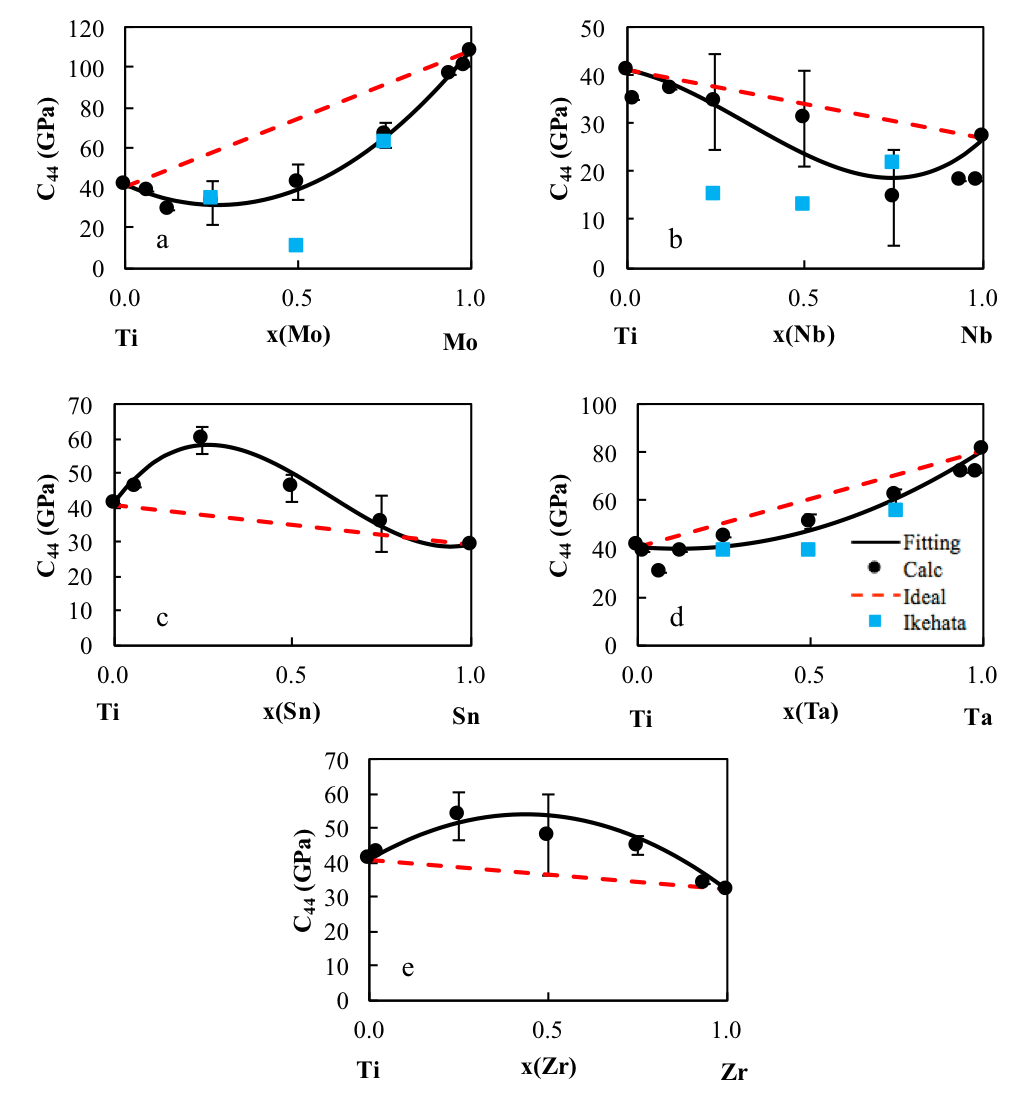
\includegraphics[width=\textwidth]{Chapter-5/Figures/tixc44.png}
	\caption{Calculated $\overline{C}_{44}$ values (circles) plotted with their errors as well as the pure element extrapolation (red dashed line) and the present modeling (black dashed line) for five Ti-X binary systems (X = Mo, Nb, Ta, Sn, Zr). Ti-Mo, Ti-Nb, and Ti-Ta alloys are compared with previous calculations from Ikehata et al. \cite{Ikehata2004}.}
	\label{Ch5-figure:tixc44}
\end{figure}

\pagebreak
\begin{figure}[H]
	\centering
	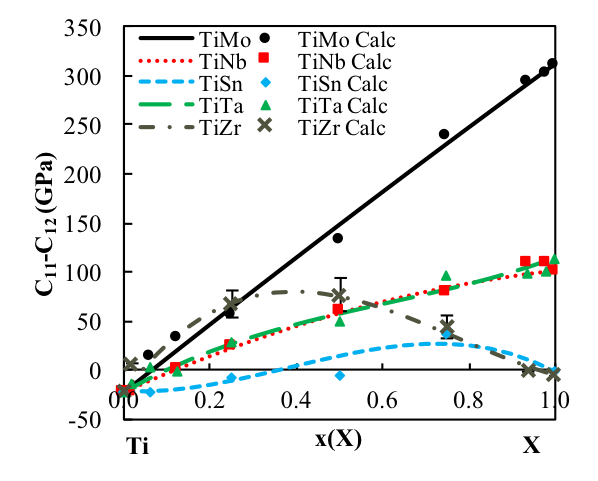
\includegraphics[width=\textwidth]{Chapter-5/Figures/tixc11-c12.png}
	\caption{Calculated $\overline{C}_{11}$-$\overline{C}_{12}$ values (circles) plotted with the present modeling (solid lines) for five Ti-X binary systems (X = Mo, Nb, Ta, Sn, Zr). The C11-C12 shows the stability of the bcc phase. When the $\overline{C}_{11}$-$\overline{C}_{12}$ value is negative the bcc phase is not stable in the corresponding compositions range.}
	\label{Ch5-figure:tixc11-c12}
\end{figure}

\pagebreak
\begin{figure}[H]
	\centering
	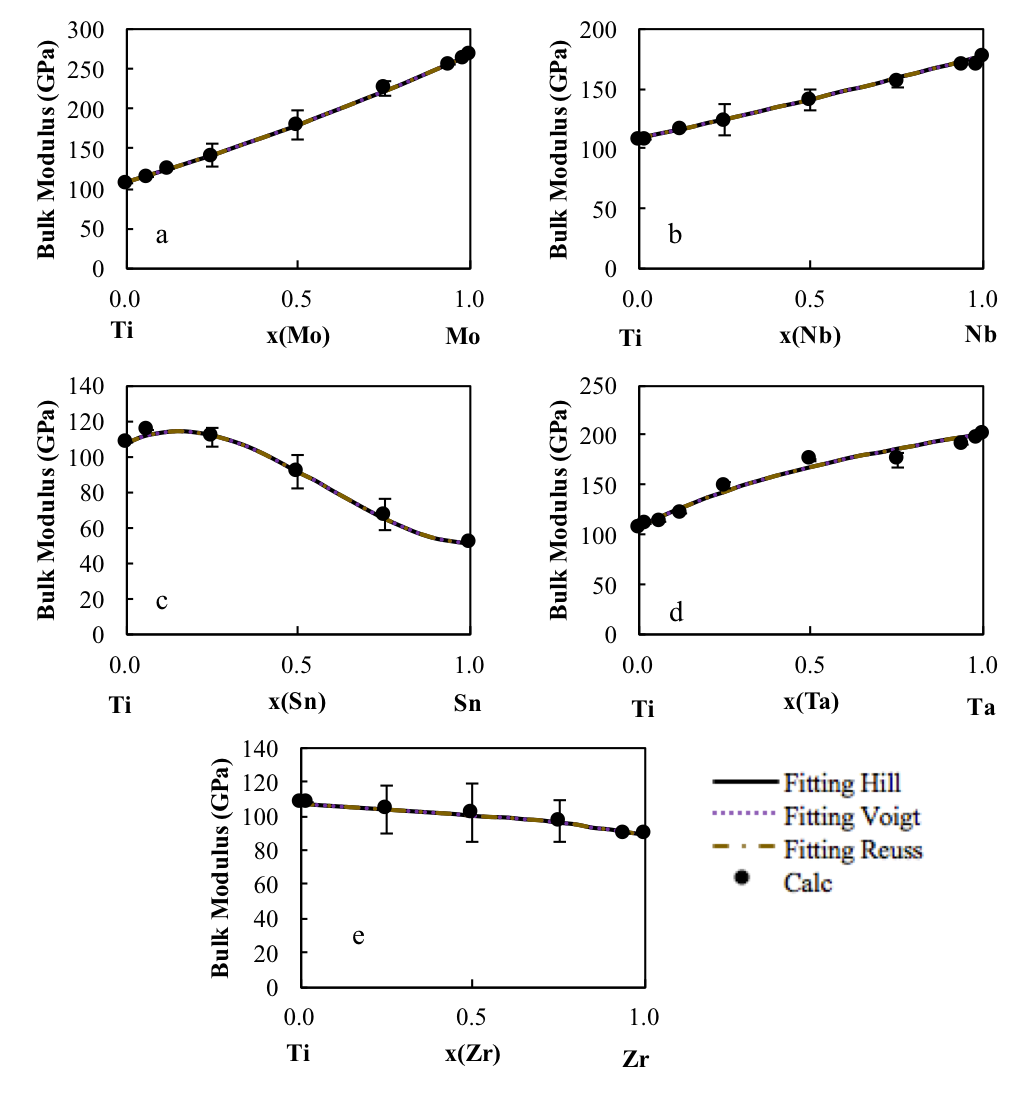
\includegraphics[width=\textwidth]{Chapter-5/Figures/tixbulk.png}
	\caption{Bulk modulus \textit{B} of the Ti-X binary systems. The present calculations are plotted as the filled circles with the error bars. The dotted purple line is the Voigt upper bulk modulus bound, the gold dot dashed line is the lower Reuss bulk modulus bound and the black line is the Hill bulk modulus average.}
	\label{Ch5-figure:tixbulk}
\end{figure}

\pagebreak
\begin{figure}[H]
	\centering
	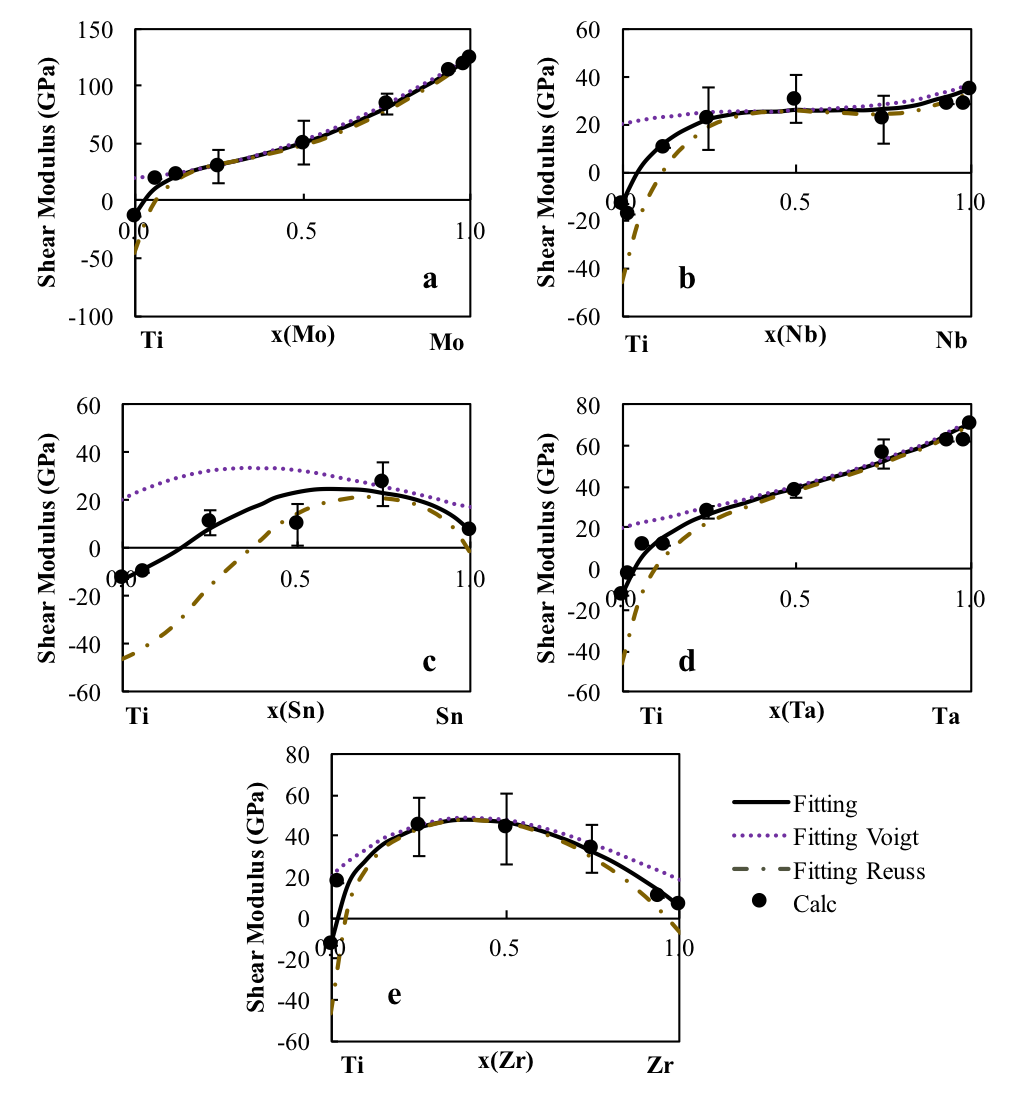
\includegraphics[width=\textwidth]{Chapter-5/Figures/tixshear.png}
	\caption{Shear modulus \textit{G} of the Ti-X binary systems. The present calculations are plotted as the filled circles with the error bars. The dotted purple line is the Voigt upper shear modulus bound, the gold dot dashed line is the lower Reuss shear modulus bound and the black line is the Hill shear modulus average.}
	\label{Ch5-figure:tixshear}
\end{figure}

\pagebreak
\begin{figure}[H]
	\centering
	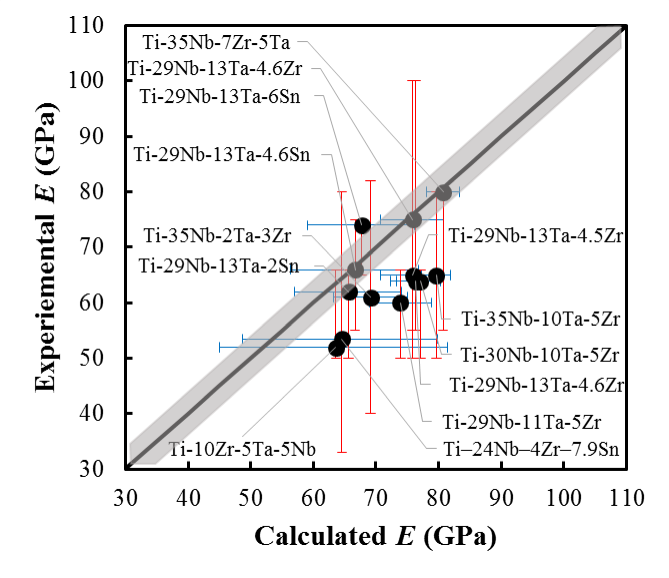
\includegraphics[width=\textwidth]{Chapter-5/Figures/edatabase.png}
	\caption{Young's modulus values of multicomponent bcc Ti alloys measured experimentally plotted against the predicted Young's modulus from the pure elements and binary interaction parameters with the black diagonal line showing the exact correlation between the experimental and calculated values. Error bars in the experiments and the bounds from Reuss and Voigt approximations are plotted as vertical and horizontal lines, respectively. The variance in the first calculations from Eq. Y-Eq. Y was averaged and plotted as the grey region to show the variance in the first-principles calculations. More information on the alloys is in Table \ref{Ch5-table:elasdata} \cite{Tane2010a,Geetha2009,Mohammed2014}}
	\label{Ch5-figure:tixdatabase}
\end{figure}